\documentclass[12pt,a4paper]{article}

% Packages
\usepackage[a4paper,top=2.5cm,bottom=2.5cm,left=2.5cm,right=2.5cm]{geometry}
\usepackage{graphicx}
\usepackage{array}
\usepackage{float}
\usepackage{setspace}
\usepackage{longtable}
\usepackage[hidelinks]{hyperref}
\usepackage{caption}
\usepackage{needspace}
\usepackage{booktabs}
\usepackage{amsmath}

% Global settings
\setstretch{1.08}
\setlength{\textfloatsep}{8pt plus 2pt minus 2pt}
\setlength{\intextsep}{8pt plus 2pt minus 2pt}
\setlength{\abovecaptionskip}{4pt}
\setlength{\belowcaptionskip}{2pt}
\graphicspath{{./}{resultImage/}{image/}}
\newcommand{\sectionbreakguard}{\Needspace{8\baselineskip}}
\newcommand{\subsectionbreakguard}{\Needspace{5\baselineskip}}

% Centered column helper
\newcolumntype{C}[1]{>{\centering\arraybackslash}p{#1}}

% Document
\begin{document}

\begin{titlepage}
\centering

% Logos
\begin{minipage}[c]{0.44\textwidth}
  \raggedright
  
\includegraphics[width=3cm]{image/ITC_Tran_Logo.png}
\end{minipage}%
\hfill%
\begin{minipage}[c]{0.44\textwidth}
  \raggedleft
  
\includegraphics[width=3cm]{image/AMS-Logo.jpg}
\end{minipage}

\vspace{0.5cm}
\noindent\rule{\linewidth}{0.8pt}
\vspace{0.3cm}

% Institution
{\Large\bfseries INSTITUTE OF TECHNOLOGY OF CAMBODIA\par}

\vspace{0.25cm}

{\large\bfseries Department of Applied Mathematics and Statistics\par}

\vspace{0.2cm}
\noindent\rule{\linewidth}{0.4pt}
\vspace{1.2cm}

% Course
{\large\bfseries Probabilistic Graphical Models\par}

\vspace{0.3cm}

{\normalsize I4-AMS-DAS-A \quad (2025--2026)\par}

\vspace{1.5cm}

% Project title
{\LARGE\bfseries Building a Robust Part-of-Speech Tagger using Hidden Markov Model\par}

\vspace{1.8cm}

% Team table
{\large\bfseries Team 3\par}
\vspace{0.5cm}

\renewcommand{\arraystretch}{1.4}
\begin{tabular}{C{6.5cm} C{3.8cm} C{2cm}}
  \toprule
  \textbf{Name of Student} & \textbf{Student ID} & \textbf{Score} \\
  \midrule
  1.\enspace HEAM VISAL    & e20221349           & \dots \\
  \bottomrule
\end{tabular}

\vfill

% Footer
\noindent\rule{\linewidth}{0.4pt}\\[6pt]
\begin{minipage}[t]{0.55\textwidth}
  \raggedright
  \begin{tabular}{@{}l@{\enspace}l@{}}
    \textbf{Lecturer:} & Mr. PHOK Ponna \\
                       & Mr. PHOK Ponna \\
  \end{tabular}
\end{minipage}%
\hfill%
\begin{minipage}[t]{0.40\textwidth}
  \raggedleft
  (Course)\\
  (TP)
\end{minipage}

\end{titlepage}

\clearpage

\section{Abstract}

This report presents a Part-of-Speech (POS) tagger based on a Hidden Markov Model
(HMM). The system was implemented from scratch and evaluated on the Brown Corpus
from NLTK using the universal POS tagset. The task is to assign the most likely
POS tag to each word in a sentence. The dataset contains 57,340 sentences and was
divided into 80\% training data and 20\% testing data. The HMM parameters were
estimated using Maximum Likelihood Estimation from frequency counts. To handle
unseen words, Laplace smoothing with $\alpha = 1.0$ and a special
\texttt{\textless OOV\textgreater} token were used. The Viterbi algorithm was
implemented in log-space to avoid numerical underflow. On the test set, the model
tagged 217,777 out of 232,177 words correctly, giving an accuracy of 93.8\%.
The results show that a simple statistical sequence model can achieve strong
performance for POS tagging, although errors remain for ambiguous and unseen
words.

\section{Introduction}

Part-of-Speech tagging is a basic task in Natural Language Processing (NLP). It
assigns a grammatical category, such as noun, verb, adjective, or adposition, to
each word in a sentence. POS tagging is useful because it provides syntactic
information for many later NLP tasks, including parsing, information extraction,
machine translation, and text analysis.

This mini project builds a POS tagger using a Hidden Markov Model. An HMM is a
probabilistic model for sequence data. In this task, the observed sequence is the
sentence, and the hidden sequence is the POS tag sequence. The model assumes that
each tag depends mainly on the previous tag, and that each word is generated from
its tag.

The project uses the Brown Corpus from NLTK with the universal POS tagset. The
universal tagset reduces the original detailed tag labels into 12 general POS
tags. This makes the task simpler and allows the model to focus on common
grammatical categories. The main objective is to train the HMM from the training
sentences and use it to predict POS tags for unseen test sentences.

\section{Methodology}

\subsection{Dataset and Tagset}

The dataset used in this project is the Brown Corpus provided by NLTK. The
corpus was loaded with the universal POS tagset. In total, the dataset contains
57,340 tagged sentences. The data was split into 45,872 training sentences and
11,468 testing sentences, following an 80\%--20\% split. The vocabulary size in
the training data is 45,153, and the number of POS tags is 12.

\begin{figure}[H]
    \centering
    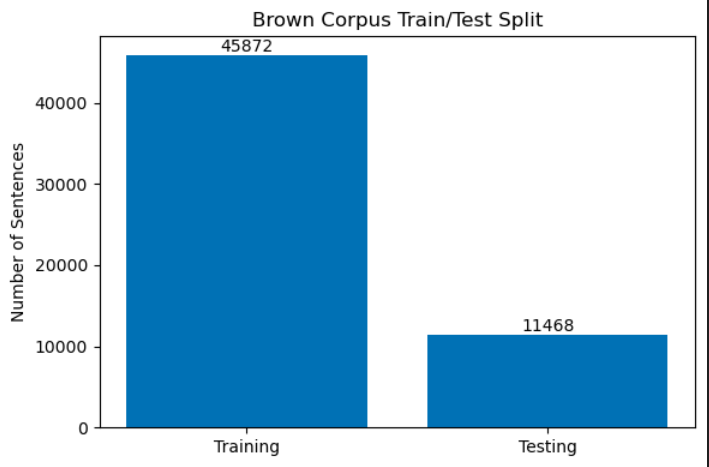
\includegraphics[width=0.72\linewidth, trim=0 0 14pt 0, clip]{Dataset-split-result.png}
    \caption{Dataset split between training and testing sentences.}
    \label{fig:dataset-split}
\end{figure}

\subsection{Hidden Markov Model}

The POS tagging problem is modeled as a sequence prediction problem. Given a
sentence $w_1, w_2, \ldots, w_n$, the goal is to find the most likely tag sequence
$t_1, t_2, \ldots, t_n$. The HMM represents the joint probability of the tag and
word sequence as:

\begin{equation}
P(t_1, \ldots, t_n, w_1, \ldots, w_n)
= \pi(t_1) B_{t_1}(w_1)
\prod_{i=2}^{n} A_{t_{i-1},t_i} B_{t_i}(w_i)
\end{equation}

In this formula, $\pi$ is the initial probability, $A$ is the transition
probability matrix, and $B$ is the emission probability matrix. These parameters
are estimated from the training data.

\subsection{Parameter Estimation}

The model parameters were estimated using Maximum Likelihood Estimation based on
frequency counts. The initial probability estimates how likely a tag is to start
a sentence:

\begin{equation}
\pi(t) = \frac{\text{Count}(t \text{ starts a sentence})}
{\text{Total sentences}}
\end{equation}

The transition probability estimates how likely tag $j$ is to follow tag $i$:

\begin{equation}
A(i,j) = \frac{\text{Count}(\text{tag}_i \text{ followed by } \text{tag}_j)}
{\text{Count}(\text{tag}_i)}
\end{equation}

The emission probability estimates how likely word $w$ is generated by tag $t$.
Laplace smoothing was used to reduce zero-probability problems:

\begin{equation}
B(t,w) = \frac{\text{Count}(w \text{ emitted by } t) + \alpha}
{\text{Count}(t) + \alpha |V|}
\end{equation}

In this project, $\alpha = 1.0$. A special
\texttt{\textless OOV\textgreater} token was used for unseen words. During
testing, words not found in the training vocabulary were treated as OOV words.

\subsection{Decoding with Viterbi Algorithm}

After estimating the HMM parameters, the Viterbi algorithm was used to find the
best tag sequence for each test sentence. The algorithm uses dynamic programming
to avoid checking all possible tag sequences directly. Since multiplying many
small probabilities can cause computational underflow, the implementation uses
log-space. The recurrence is:

\begin{equation}
\log v_t(j) =
\max_i \left[\log v_{t-1}(i) + \log A(i,j)\right]
+ \log B(j,w_t)
\end{equation}

The model stores the best previous tag for each current tag and then performs
backtracking to recover the predicted tag sequence.

\section{Results and Evaluation}

\subsection{Evaluation Metric}

The model was evaluated using word-level accuracy. Accuracy measures the
proportion of test words whose predicted POS tag is equal to the true POS tag:

\begin{equation}
\text{Accuracy} =
\frac{\text{Correctly tagged words}}{\text{Total test words}}
\end{equation}

\subsection{Final Evaluation Summary}

Table~\ref{tab:summary} shows the final evaluation summary. The model achieved
93.8\% accuracy on 232,177 test words. Out of these words, 217,777 were tagged
correctly and 14,400 were tagged incorrectly.

\begin{table}[H]
    \centering
    \caption{Final Evaluation Summary}
    \label{tab:summary}
    \begin{tabular}{lr}
        \toprule
        \textbf{Metric} & \textbf{Value} \\
        \midrule
        Training sentences & 45,872 \\
        Testing sentences & 11,468 \\
        Vocabulary size & 45,153 \\
        POS tags & 12 \\
        Total test words & 232,177 \\
        Correct words & 217,777 \\
        Wrong words & 14,400 \\
        Accuracy & 93.8\% \\
        OOV words & 5,050 \\
        OOV rate & 2.18\% \\
        \bottomrule
    \end{tabular}
\end{table}

\begin{figure}[H]
    \centering
    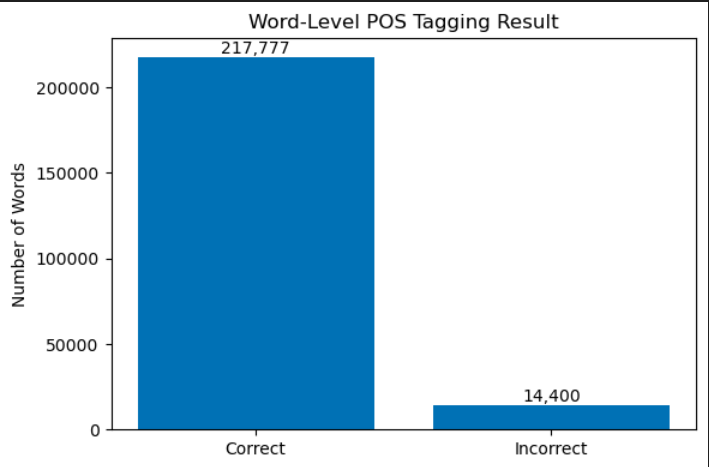
\includegraphics[width=0.72\linewidth, trim=0 0 13pt 0, clip]{Final-accuracy-result-with-numbers-on-bars.png}
    \caption{Word-level POS tagging result on the test set.}
    \label{fig:word-result}
\end{figure}

\subsection{OOV Analysis}

The test set contains 5,050 OOV words, giving an OOV rate of 2.18\%. OOV words
are words that do not appear in the training vocabulary. The model handles these
words using Laplace smoothing and the \texttt{\textless OOV\textgreater} token.
This allows the model to assign non-zero emission probabilities to unseen words.
However, OOV words are still difficult because the model has no direct training
evidence for their most likely tags.

\begin{figure}[H]
    \centering
    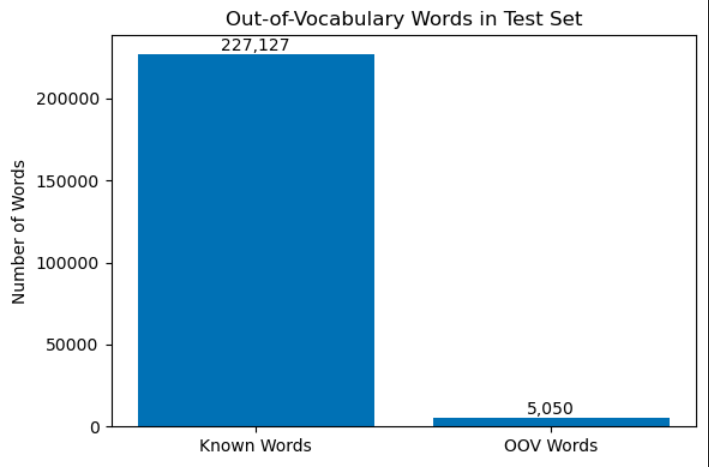
\includegraphics[width=0.72\linewidth, trim=0 0 13pt 0, clip]{OOV-analysis-result-with-numbers-on-bars.png}
    \caption{OOV word analysis on the test set.}
    \label{fig:oov-analysis}
\end{figure}

\begin{figure}[H]
    \centering
    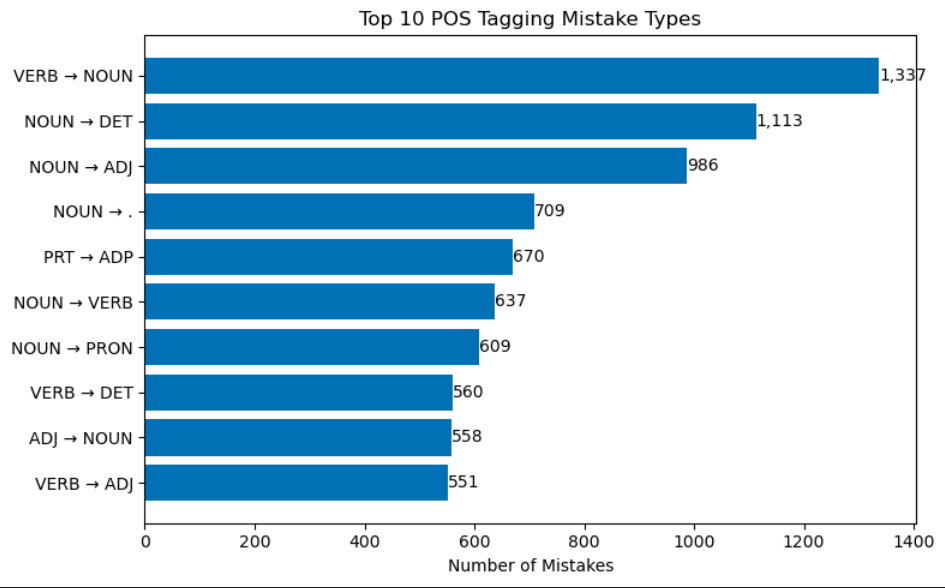
\includegraphics[width=0.78\linewidth]{Top-10-mistake-types-with-numbers-on-bars.png}
    \caption{Top 10 POS tagging mistake types.}
    \label{fig:top-mistakes}
\end{figure}

\section{Error Analysis}

The model made 14,400 word-level mistakes on the test set. Many mistakes happen
because some English words are ambiguous. A word can have different POS tags
depending on how it is used in a sentence. For example, ``average'' can be a
noun, adjective, or verb depending on context. Similarly, ``offer'' can be a noun
or a verb.

Table~\ref{tab:error-examples} shows selected failed examples from the test
sentences.

\begin{table}[H]
    \centering
    \caption{Error Analysis Examples}
    \label{tab:error-examples}
    \small
    \begin{tabular}{p{0.40\textwidth}p{0.14\textwidth}p{0.14\textwidth}p{0.20\textwidth}}
        \toprule
        \textbf{Sentence} & \textbf{Word} & \textbf{True Tag} & \textbf{Predicted Tag} \\
        \midrule
        With tips, the girls average between \$150 and \$200 a week, depending on basic salary.
        & average & VERB & NOUN \\
        & \$200 & NOUN & ADP \\
        & depending & ADP & VERB \\
        \midrule
        It was a very tempting offer.
        & very & ADV & ADJ \\
        & tempting & VERB & NOUN \\
        & offer & NOUN & VERB \\
        \midrule
        He saw the surprise in her face, and laughed as though it were the funniest expression he had ever seen.
        & as & ADP & ADV \\
        \bottomrule
    \end{tabular}
\end{table}

The HMM uses the first-order Markov assumption. This means that the current tag
mainly depends on the previous tag, not on the full meaning of the sentence.
Because of this, the model may fail when the correct tag requires longer context
or semantic understanding. For example, deciding whether ``offer'' is a noun or a
verb may require understanding its role in the sentence, not only the previous
tag.

Rare words and unseen words are also challenging. Laplace smoothing helps by
preventing zero probabilities, but it cannot fully replace real evidence from
training data. Therefore, OOV words can still receive incorrect tags, especially
when they appear in unusual contexts.

\section{Conclusion}

This project implemented a POS tagger using a Hidden Markov Model trained on the
Brown Corpus with the universal POS tagset. The model estimated initial,
transition, and emission probabilities from frequency counts using Maximum
Likelihood Estimation. Laplace smoothing with $\alpha = 1.0$ and a
\texttt{\textless OOV\textgreater} token were used to handle unseen words. The
Viterbi algorithm was implemented in log-space to decode the most likely POS tag
sequence while avoiding computational underflow.

The final result shows that the HMM POS tagger achieved 93.8\% accuracy on the
test set. This is a strong result for a simple statistical model built from
scratch. The main weaknesses are related to ambiguous words, limited context from
the first-order Markov assumption, and rare or unseen words. Future improvements
could include using richer word features, suffix information, higher-order tag
dependencies, or modern neural sequence models.

\begin{thebibliography}{9}

\bibitem{nltkbook}
Steven Bird, Ewan Klein, and Edward Loper.
\textit{Natural Language Processing with Python: Analyzing Text with the Natural Language Toolkit}.
O'Reilly Media, 2009. Official online version available at
\url{https://www.nltk.org/book/}.

\bibitem{nltkcorpus}
NLTK Project.
\textit{NLTK Corpus Reader Documentation}.
Official documentation showing access to the Brown Corpus and the universal POS
tagset. Available at \url{https://www.nltk.org/howto/corpus.html}.

\bibitem{viterbi}
Andrew J. Viterbi.
Error bounds for convolutional codes and an asymptotically optimum decoding
algorithm.
\textit{IEEE Transactions on Information Theory}, 13(2):260--269, 1967.
DOI: \url{https://doi.org/10.1109/TIT.1967.1054010}.

\bibitem{rabiner}
Lawrence R. Rabiner.
A tutorial on hidden Markov models and selected applications in speech
recognition.
\textit{Proceedings of the IEEE}, 77(2):257--286, 1989.
DOI: \url{https://doi.org/10.1109/5.18626}.

\end{thebibliography}

\end{document}
